% ISBI 2027 4-page paper, draft of 2 November 2026 (brain MRI only). Template: ISBI_template-master (spconf.sty, IEEEbib.bst).
\documentclass{article}
\usepackage{spconf,amsmath,amssymb,graphicx}
\usepackage{booktabs}
\usepackage[hidelinks]{hyperref}
\usepackage{enumitem}
\setlist{nosep, leftmargin=12pt}
\newtheorem{prop}{Proposition}
\newcommand{\todo}[1]{\textbf{[#1]}}
\raggedbottom

\title{Fighting regression to the mean in the evaluation of brain MRI inpainting}
\name{Ekaterina Kondrateva$^{1,2}$, Florian Kofler$^{1,3,4,5}$}
\address{$^{1}$Hertie Institute for AI in Brain Health, University of T\"ubingen, T\"ubingen, Germany\\
$^{2}$Department of Radiation Oncology (Maastro), GROW, Maastricht University,\\
Maastricht, The Netherlands\\
$^{3}$AI for Image-Guided Diagnosis and Therapy, TUM School of Medicine and Health,\\
Technical University of Munich, Munich, Germany\\
$^{4}$Department of Quantitative Biomedicine, University of Zurich, Zurich, Switzerland\\
$^{5}$Helmholtz AI, Helmholtz Munich, Neuherberg, Germany\\
ORCID: E.~Kondrateva 0000-0003-3623-6106; F.~Kofler 0000-0003-0642-7884}

\begin{document}
\maketitle

\begin{abstract}
The BraTS inpainting challenge ranks algorithms for healthy-tissue inpainting in brain MRI by SSIM, PSNR and RMSE.
Even top-ranked challenge algorithms produce visibly blurred infills.
We demonstrate that this is a consequence of the ranking metrics.
Writing tissue as a population mean plus an individual part, the mean fill has half the squared error of another person's tissue and beats every donor whose individual part correlates with the target's by less than $1/2$, a sibling included.
We test this on T1 scans of 221 young adults from a twin and sibling study, filling cubes of brain tissue from each kind of donor.
One stranger's tissue had $1.98$ times the error of the dataset mean (predicted $2$), a sibling's $1.82$, the person's own mirrored hemisphere $1.49$, and only the same person's second scan beat the mean ($0.30$); the results held over seeds, cube sizes and positions.
Dice against the oracle segmentation has the same property with the mode in place of the mean.
We propose the population-mean fill as a mandatory baseline and plausibility measures that do not reward averaging.
\end{abstract}
\begin{keywords}
inpainting, image synthesis, metric validation, regression to the mean, BraTS
\end{keywords}

\section{Introduction}
\label{sec:intro}
The BraTS challenge on local synthesis of healthy brain tissue asks participants to fill masked healthy regions of T1 scans, and ranks them case-wise by SSIM, PSNR and RMSE inside the mask~\cite{kofler2023brats,inpainting2026}.
In the 2023 edition the ranking was clear, yet the organisers report that, apart from one 2D diffusion model with stripe artefacts in the orthogonal views, the submissions produced blurry inpaintings in all three views, and that qualitative inspection gave a more varied picture than the ranking~\cite{kofler2023brats}.
They called for synthesis metrics closer to expert perception.
The 2025 winner is a U-Net trained to inpaint masked regions~\cite{zhang2025brats}.

A natural remedy is to judge fills by what they are for: segment the inpainted brain with a downstream U-Net and compare the result with the segmentation of the real image.
Yet such a check scores the segmentation by Dice against the oracle, itself a pointwise score, and we show that it favours averaged fills for the same reason.

We argue that both observations follow from the metrics, not from the models.
Squared error is minimised by the conditional mean, so when the visible context carries little information about the individual anatomy inside the mask, the optimal fill is close to the population average: regression to the mean.
Pointwise label agreement is maximised by the most probable label, so a segmentation of an averaged fill lands on the population-typical boundary.
Our contributions are (i) closed forms that place the population-mean fill, averages of $k$ people and real tissue from the same person, relatives and strangers on one scale; (ii) the analogue for Dice and accuracy against the oracle; (iii) a test on real brain MRI of twins and siblings, where every fill is real tissue from a known donor, with its robustness to seeds, mask size and position; (iv) lessons from fields that faced the same problem, turned into a reporting protocol.

\begin{figure*}[t]
\centering
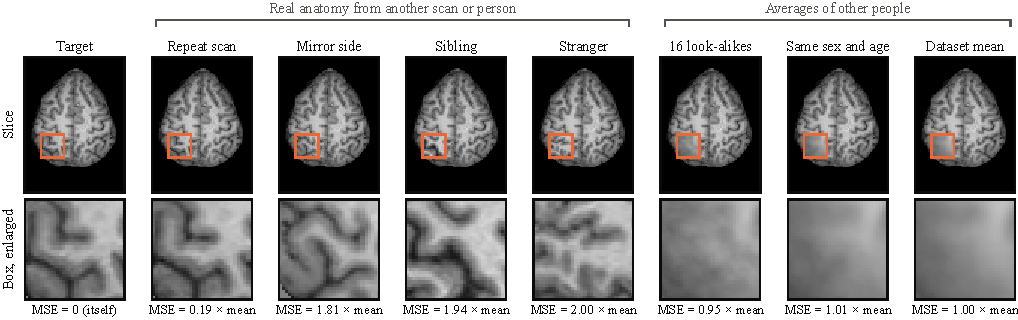
\includegraphics[width=\textwidth]{fig_real_case.pdf}
\caption{One QTIM brain, its parietal box filled from each kind of donor, from the most related to the least (axial slice, $z=55$\,mm, subject's left on the left; bottom: box enlarged).
Numbers: MSE in units of the error of the dataset mean, averaged over the 192 people whose box lies inside the brain.
Dataset mean: all unrelated participants (median 191); same sex and age: those of the same sex and an age within 2 years (median 51); look-alikes: the 16 with the most similar surrounding tissue.
The blurred averages beat the real, related tissue of a sibling and of the person's own other hemisphere; only the repeat scan wins.}
\label{fig:case}
\end{figure*}

\section{Theory}
\label{sec:theory}
Write the voxels of a masked region of person $p$ in session $s$ as $x=\mu+g_p+e_p+\eta_{ps}+\varepsilon$: population mean $\mu$, genotype $g$ (shared with correlation $1/2$ by siblings), individual development $e$, session nuisance $\eta$ and noise $\varepsilon$, independent and zero-mean, with variances per voxel.
The individual part $\delta=x-\mu$ has variance $V$, and we express every error in units of $V$, the expected squared error of the population mean itself.

\begin{prop}[squared error]
For a region of $x$ filled with $f$, the expected mean squared error divided by $V$ is $1$ for the population mean, $2$ for one stranger's tissue, and $2(1-r)$ for tissue whose individual part, of the same variance, correlates by $r$ with the target's; a sibling has $r=h^2/2$, with $h^2$ the genetic share of $V$.
An average of $k$ unrelated people drawn from a group whose own mean explains a share $R^2$ of $V$ has $(1-R^2)(1+1/k)$.
Hence the identity-free mean beats any single donor with $r<1/2$, every sibling included, although the sibling carries the share $r$ of the target's individual part and the mean carries none.
\end{prop}
\noindent The parts add because they are independent: the mean misses the target's $\delta$ (error $V$); a stranger misses it and adds its own, unrelated $\delta'$ ($V+V$); an average of $k$ strangers shrinks the added part to $V/k$.
More generally, for any predictor $f$ of the masked region from the visible context $z$, $\mathbb{E}\|x-f(z)\|^2$ is minimised by $\mathbb{E}[x\mid z]$.
If $z$ is nearly independent of the individual part inside the mask, the optimum is close to $\mu$, so a network trained on squared error, or selected by RMSE and PSNR, is pulled towards the average: a blurred fill is the expected answer, not a failure of optimisation.

\begin{prop}[pointwise label agreement]
Let a voxel belong to a tissue class with probability $p$ given the context.
A fill whose segmentation takes the most probable label agrees with the true label with probability $\max(p,1-p)$; an independent donor agrees with probability $p^2+(1-p)^2\le\max(p,1-p)$.
Expected voxel accuracy, and Dice in the same way, against the oracle segmentation therefore favour the mode over any donor that does not share the target's anatomy.
\end{prop}
\noindent A segmenter applied to a blurred fill tends to place boundaries where they are most common in the population, so a downstream Dice check inherits the bias of the intensity metrics.

\textbf{SSIM and the ranking.} For a fill that is constant within an SSIM window, $\mathrm{SSIM}=l\cdot C_2/(\sigma_x^2+C_2)$~\cite{wang2004}, with $C_2=(0.03L)^2$ and data range $L$, so where the local SD of the reference is well below $0.03L$ a mean-matched flat fill scores close to 1.
In the challenge code~\cite{inpainting2026} the PSNR data range comes from the reference inside the mask, so within a case PSNR repeats the RMSE order, and a case-wise rank-sum over SSIM, PSNR and RMSE~\cite{kofler2023brats} gives squared error two thirds of the weight.

\begin{figure*}[t]
\centering
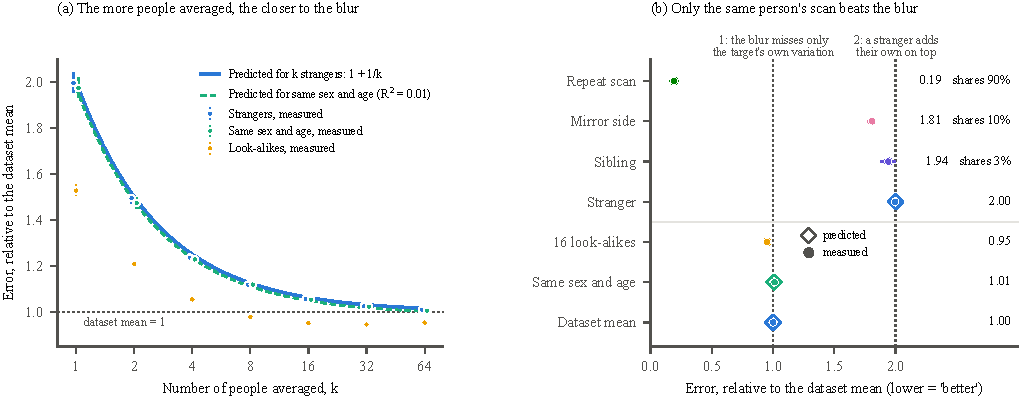
\includegraphics[width=0.88\textwidth]{fig_real_theory.pdf}
\caption{The parietal box of Fig.~\ref{fig:case} against Proposition~1.
(a) Averages of $k$ people: prediction $1+1/k$ for strangers (blue) and $(1-R^2)(1+1/k)$ with the measured $R^2=0.01$ for same sex and age (green). Look-alikes, chosen for similar context, share part of the target's pattern and have no closed form.
(b) Every column of Fig.~\ref{fig:case} with $95\%$ intervals; diamonds: predictions; right: the share $r$ each related donor has in common with the target.}
\label{fig:theory}
\end{figure*}

\section{Experiments}
\label{sec:experiments}
\textbf{Data.} Queensland Twin IMaging (QTIM)~\cite{qtim2026}: T1 scans of 221 young adults (aged 20 to 29, median 23; 125 women) from 168 families; 102 of them have a sibling of a different age in the data (49 families), and 23 have a second session from the test-retest subsample.
Every scan was bias-corrected with N4~\cite{tustison2010}, skull-stripped with SynthStrip~\cite{hoopes2022} and registered affinely with ANTs~\cite{avants2008} to the symmetric MNI ICBM 2009a template~\cite{fonov2009} on a 1\,mm grid, then z-scored inside its own brain mask.
No nonlinear registration was used for the main results, so that individual folding is not pulled towards the template.

\textbf{Masks.} 32 cubes of $16$\,mm, placed at random among template positions whose $24$\,mm window lies at least $90\%$ inside the template brain, and two fixed boxes: a deep box over the basal ganglia and thalamus ($32\times32\times24$\,mm) and a parietal cortical box (same size, $x$ from $-45$ to $-13$, $y$ from $-65$ to $-33$, $z$ from $43$ to $67$\,mm).
A mask counts for a scan when at least $95\%$ of it lies inside that scan's brain mask.

\textbf{Fills.} Each mask of each first-session scan was filled with real tissue: the same person's second session (\emph{repeat scan}); the person's other hemisphere, mirrored across the midline (\emph{mirror side}); a sibling of a different age (\emph{sibling}); one random person from another family (\emph{stranger}); the voxel-wise average of $k\in\{1,\dots,64\}$ random people from other families and of all of them (\emph{dataset mean}); the same restricted to people of the same sex and an age within 2 years (\emph{same sex and age}); and the average of the $k$ people whose $4$\,mm shell of tissue around the mask is closest to the target's (\emph{look-alikes}).
Every pool excludes the target's whole family.

\textbf{Measures.} For each target and mask we compute the mean squared error of the fill inside the mask and divide the mean over targets by the same mean for the dataset mean, so that the dataset mean scores $1$ and Proposition~1 predicts $2$ for one stranger.
For single donors we report $r=1-\mathrm{ratio}/2$, the share of the individual part they have in common with the target.
For the averages we fit $(1-R^2)(1+1/k)$ over $k$.
Intervals are $95\%$ percentiles of 2000 bootstrap resamples of families.
To test robustness we repeated the analysis with five more seeds for cube positions and donor draws, with cubes of $12$, $24$ and $32$\,mm, with other thresholds for the template and scan masks, and on a fixed subset (every person with a second session and 15 sibling pairs) with SyN registration~\cite{avants2008} added on top of the affine one.
The protocol was written before any result of each run was looked at.

\section{Results}
\label{sec:results}

\begin{table}[t]
\centering
\caption{Mean squared error of each fill in units of the error of the dataset mean, with $95\%$ intervals (family bootstrap). Random cubes: 32 cubes of 16\,mm.}
\label{tab:fills}
\footnotesize
\setlength{\tabcolsep}{2.5pt}
\begin{tabular}{@{}lccc@{}}
\toprule
Fill & random cubes & deep box & parietal box \\
\midrule
repeat scan & 0.30 [0.22, 0.40] & 0.33 [0.17, 0.54] & 0.19 [0.16, 0.23] \\
mirror side & 1.49 [1.46, 1.51] & 0.63 [0.58, 0.69] & 1.81 [1.77, 1.84] \\
sibling & 1.82 [1.78, 1.86] & 1.86 [1.63, 2.08] & 1.94 [1.88, 2.00] \\
stranger (pred.\ 2) & 1.98 [1.96, 2.01] & 2.06 [1.90, 2.23] & 2.00 [1.95, 2.04] \\
16 look-alikes & 0.75 & 0.45 & 0.95 \\
same sex and age & 1.01 & 0.99 & 1.01 \\
dataset mean & 1 & 1 & 1 \\
\midrule
fitted $R^2$, sex and age & 0.01 & 0.04 & 0.01 \\
\bottomrule
\end{tabular}
\end{table}

\textbf{The ladder on real tissue.} One stranger's tissue had $1.98$ times the error of the dataset mean over the random cubes, as Proposition~1 predicts, and the error of an average of $k$ strangers followed $1+1/k$ without any fitted parameter (rms deviation $0.002$; Fig.~\ref{fig:theory}a).
A sibling's tissue scored $1.82$ ($r=0.09$), close to a stranger and far behind the blurred mean (Table~\ref{tab:fills}).
The person's own other hemisphere scored $1.49$ ($r=0.26$) on average and $1.81$ in the parietal cortex, where folding is asymmetric; only in the deep box, where subcortical anatomy is nearly symmetric, did it beat the mean ($0.63$).
Only the same person's repeat scan beat the mean everywhere ($0.19$ to $0.33$, $r=0.84$ to $0.90$).
Sex and age explained $1\%$ to $4\%$ of the individual variance: averaging people of the same sex and age did no better than the dataset mean, partly because the participants' ages span only 20 to 29 years.
Look-alikes chosen by the surrounding tissue beat the mean by $5\%$ in the parietal box, $25\%$ over the random cubes and $55\%$ in the deep box, with a U-shaped error over $k$ and the best $k$ between 8 and 32.

\textbf{Robustness.} Over five further seeds the stranger's error stayed between $1.98$ and $2.00$ over the random cubes, the sibling's $r$ between $0.07$ and $0.10$, the repeat scan's between $0.84$ and $0.87$, and the mirror side's between $0.21$ and $0.39$; the $R^2$ of sex and age stayed at $0.01$.
Cubes of $12$ and $24$\,mm gave the same picture \todo{32\,mm, mask thresholds and SyN to add}.

\section{How other fields fight it}
\label{sec:fields}
In image restoration, lowering mean distortion provably makes outputs easier to tell apart from real images, so restoration is judged on distortion and perceptual quality together~\cite{blau2018}.
Deep nowcasting models trained on rain rates give blurry forecasts; a generative model was preferred by expert meteorologists~\cite{ravuri2021}, and verification over neighbourhoods credits a realistic storm placed slightly wrong~\cite{roberts2008}.
Protein structure models are scored against random pairs, with TM-score normalised so that random pairs score the same at any length~\cite{zhang2004}, and lDDT adds a plausibility check that does not reward closeness to the reference~\cite{mariani2013}.
For inpainting this gives four rules.
\begin{enumerate}
\item \textbf{The population mean is a baseline entry}, with a blurred version; a method that does not beat it on a metric has shown nothing about the individual on that metric.
\item \textbf{Report distance from the mean next to distance from the truth.}
\item \textbf{Score plausibility, not only overlap}: shape and topology of the segmentation, and population-level realism of the fill.
\item \textbf{Calibrate raw values} against fills from other people: on this scale the mean scores 1 and a stranger 2, whatever the region.
\end{enumerate}
Limitations: one dataset of young adults, affine registration whose visual quality control is not yet complete, real tissue as fills rather than challenge entries, and the label-space result shown in theory only.
\section{Compliance with ethical standards}
\label{sec:ethics}
This research study was conducted retrospectively using human subject data made available in open access by the Queensland Twin IMaging study (OpenNeuro ds004169, CC0 licence)~\cite{qtim2026}.
Ethical approval was not required as confirmed by the licence attached with the open access data.

\section{Acknowledgments}
\label{sec:acknowledgments}
This work was supported by Anna Valentina Lioba Eleonora Claire Javid Mamasani and the Gemeinn\"utzige Hertie Stiftung.
The authors declare no conflicts of interest.
GPT-6 Astra (OpenAI, high effort) in Codex helped write the MRI preparation code, and Claude Opus 5.5 (Anthropic, medium effort) the analysis code, the literature search and the draft text; E.K. re-checked every derivation, number and figure against the released results, and every reference against Crossref, DataCite or PubMed with a dedicated citation-check workflow.

\bibliographystyle{IEEEbib}
{\small\bibliography{refs}}
\end{document}
